\documentclass[11pt,a4paper]{article}
\usepackage[utf8x]{inputenc}
\usepackage[T1]{fontenc}
\usepackage{mathptmx}
\usepackage{graphicx}
\usepackage[pdftex,linkcolor=black,pdfborder={0 0 0}]{hyperref} % Format links for pdf
\usepackage{calc} % To reset the counter in the document after title page
\usepackage{enumitem} % Includes lists
\usepackage{caption}
\captionsetup[figure]{font=small,labelfont=small,labelfont=bf}
\usepackage{subcaption}
\usepackage{amsmath}
\usepackage{amssymb}
\usepackage{amsfonts}
\usepackage{fancyvrb,newverbs,xcolor}
\usepackage{verbatim}
\definecolor{cverbbg}{gray}{0.93}

\newenvironment{lcverbatim}
 {\SaveVerbatim{cverb}}
 {\endSaveVerbatim
  \flushleft\fboxrule=0pt\fboxsep=.5em
  \colorbox{cverbbg}{%
    \makebox[\dimexpr\linewidth-2\fboxsep][l]{\BUseVerbatim{cverb}}%
  }
  \endflushleft
}

\renewcommand\thesection{Task \arabic{section}}
\renewcommand\thesubsection{\alph{subsection}.)}
\renewcommand\thesubsubsection{\Roman{subsubsection}:}

\frenchspacing
\linespread{1.2}
\usepackage[a4paper, lmargin=0.12\paperwidth, rmargin=0.12\paperwidth, tmargin=0.05\paperheight, bmargin=0.1\paperheight]{geometry}

\usepackage[all]{nowidow} % Tries to remove widows
\usepackage[protrusion=true,expansion=true]{microtype}

\title{Exercise 8}
\author{Kai Schneider}
\date{\today}

\begin{document} 

\maketitle

\section{n-step and eligibility traces}

\subsection{ n-step bootstrapping or Dyna-Q}

Which algorithm performs better depends on the number of steps in the first episode.

\begin{itemize}
  \item If the \textit{first episode has \textbf{less} than n} steps both would perform the same. 
        Before reaching the goal, the algorithms can't modify their behaviour since all rewards are still equal.
        If a path is found, both have to do the same number of updates, which results in the same performance.
        Starting with the second episode, Dyna-Q should perform better due to using the information from the previous episode.

  \item If the \textit{first episode has \textbf{more} than n} steps Dyna-Q can directly update all n steps after reaching the
        goal. n-bootstrapping wouldn't be able to do this, so Dyna-Q would clearly perform better in this case. 
\end{itemize}

\flushleft
The ability to revisited all already visited states allows Dyna-Q to gain more information.
However the performance depends on the chosen environment. If the sorrounding isn't static, Dyna-Q should might 
have more issuses compared to n-step bootstrapping.

\newpage

\subsection{}

Given:

\begin{align}
    G_{t}^{\lambda} = (1-\lambda) \sum_{n=1}^{\infty} \lambda^{n-1} G_{t:t+n} \\
    G_{t:t+n} = R_{t+1} + \gamma R_{t+2} + \dots + \gamma^{n-1} R_{t+n} + \gamma^{n} V(S_{t+n})
\end{align}

Plug $(2)$ in $(1)$:

\begin{align*}
  G_{t}^{\lambda} &= (1-\lambda) \sum_{n=1}^{\infty} \lambda^{n-1} \bigl( 
  R_{t+1} + \gamma R_{t+2} + \dots + \gamma^{n-1} R_{t+n} + \gamma^{n} V(S_{t+n}) \bigr) \\
  &= (1-\lambda) \sum_{n=1}^{\infty} \lambda^{n-1}R_{t+1} + 
  (1-\lambda) \sum_{n=1}^{\infty} \lambda^{n-1}\gamma \underbrace{\bigl( R_{t+2} + 
  \gamma R_{t+3}\dots + \gamma^{n-2} R_{t+n} + \gamma^{n-1} V(S_{t+n}) \bigr)}_{ G_{t+1:t+n}} \\
  &= (1-\lambda) \sum_{n=1}^{\infty} \lambda^{n-1}R_{t+1} +
  (1-\lambda) \sum_{n=1}^{\infty} \lambda^{n-1}\gamma G_{t+1:t+n} \\
  &= (1-\lambda) \sum_{n=1}^{\infty} \lambda^{n-1}R_{t+1} +
  \gamma \underbrace{(1-\lambda) \sum_{n=1}^{\infty} \lambda^{n-1} G_{t+1:t+n}}_{G_{t+1}^{\lambda}} \\
  &= (1-\lambda) \sum_{n=1}^{\infty} \lambda^{n-1} R_{t+1} + \gamma G_{t+1}^{\lambda}
\end{align*}

\vspace{20pt}


\section{n-step sarsa}

\begin{figure}[h!]
  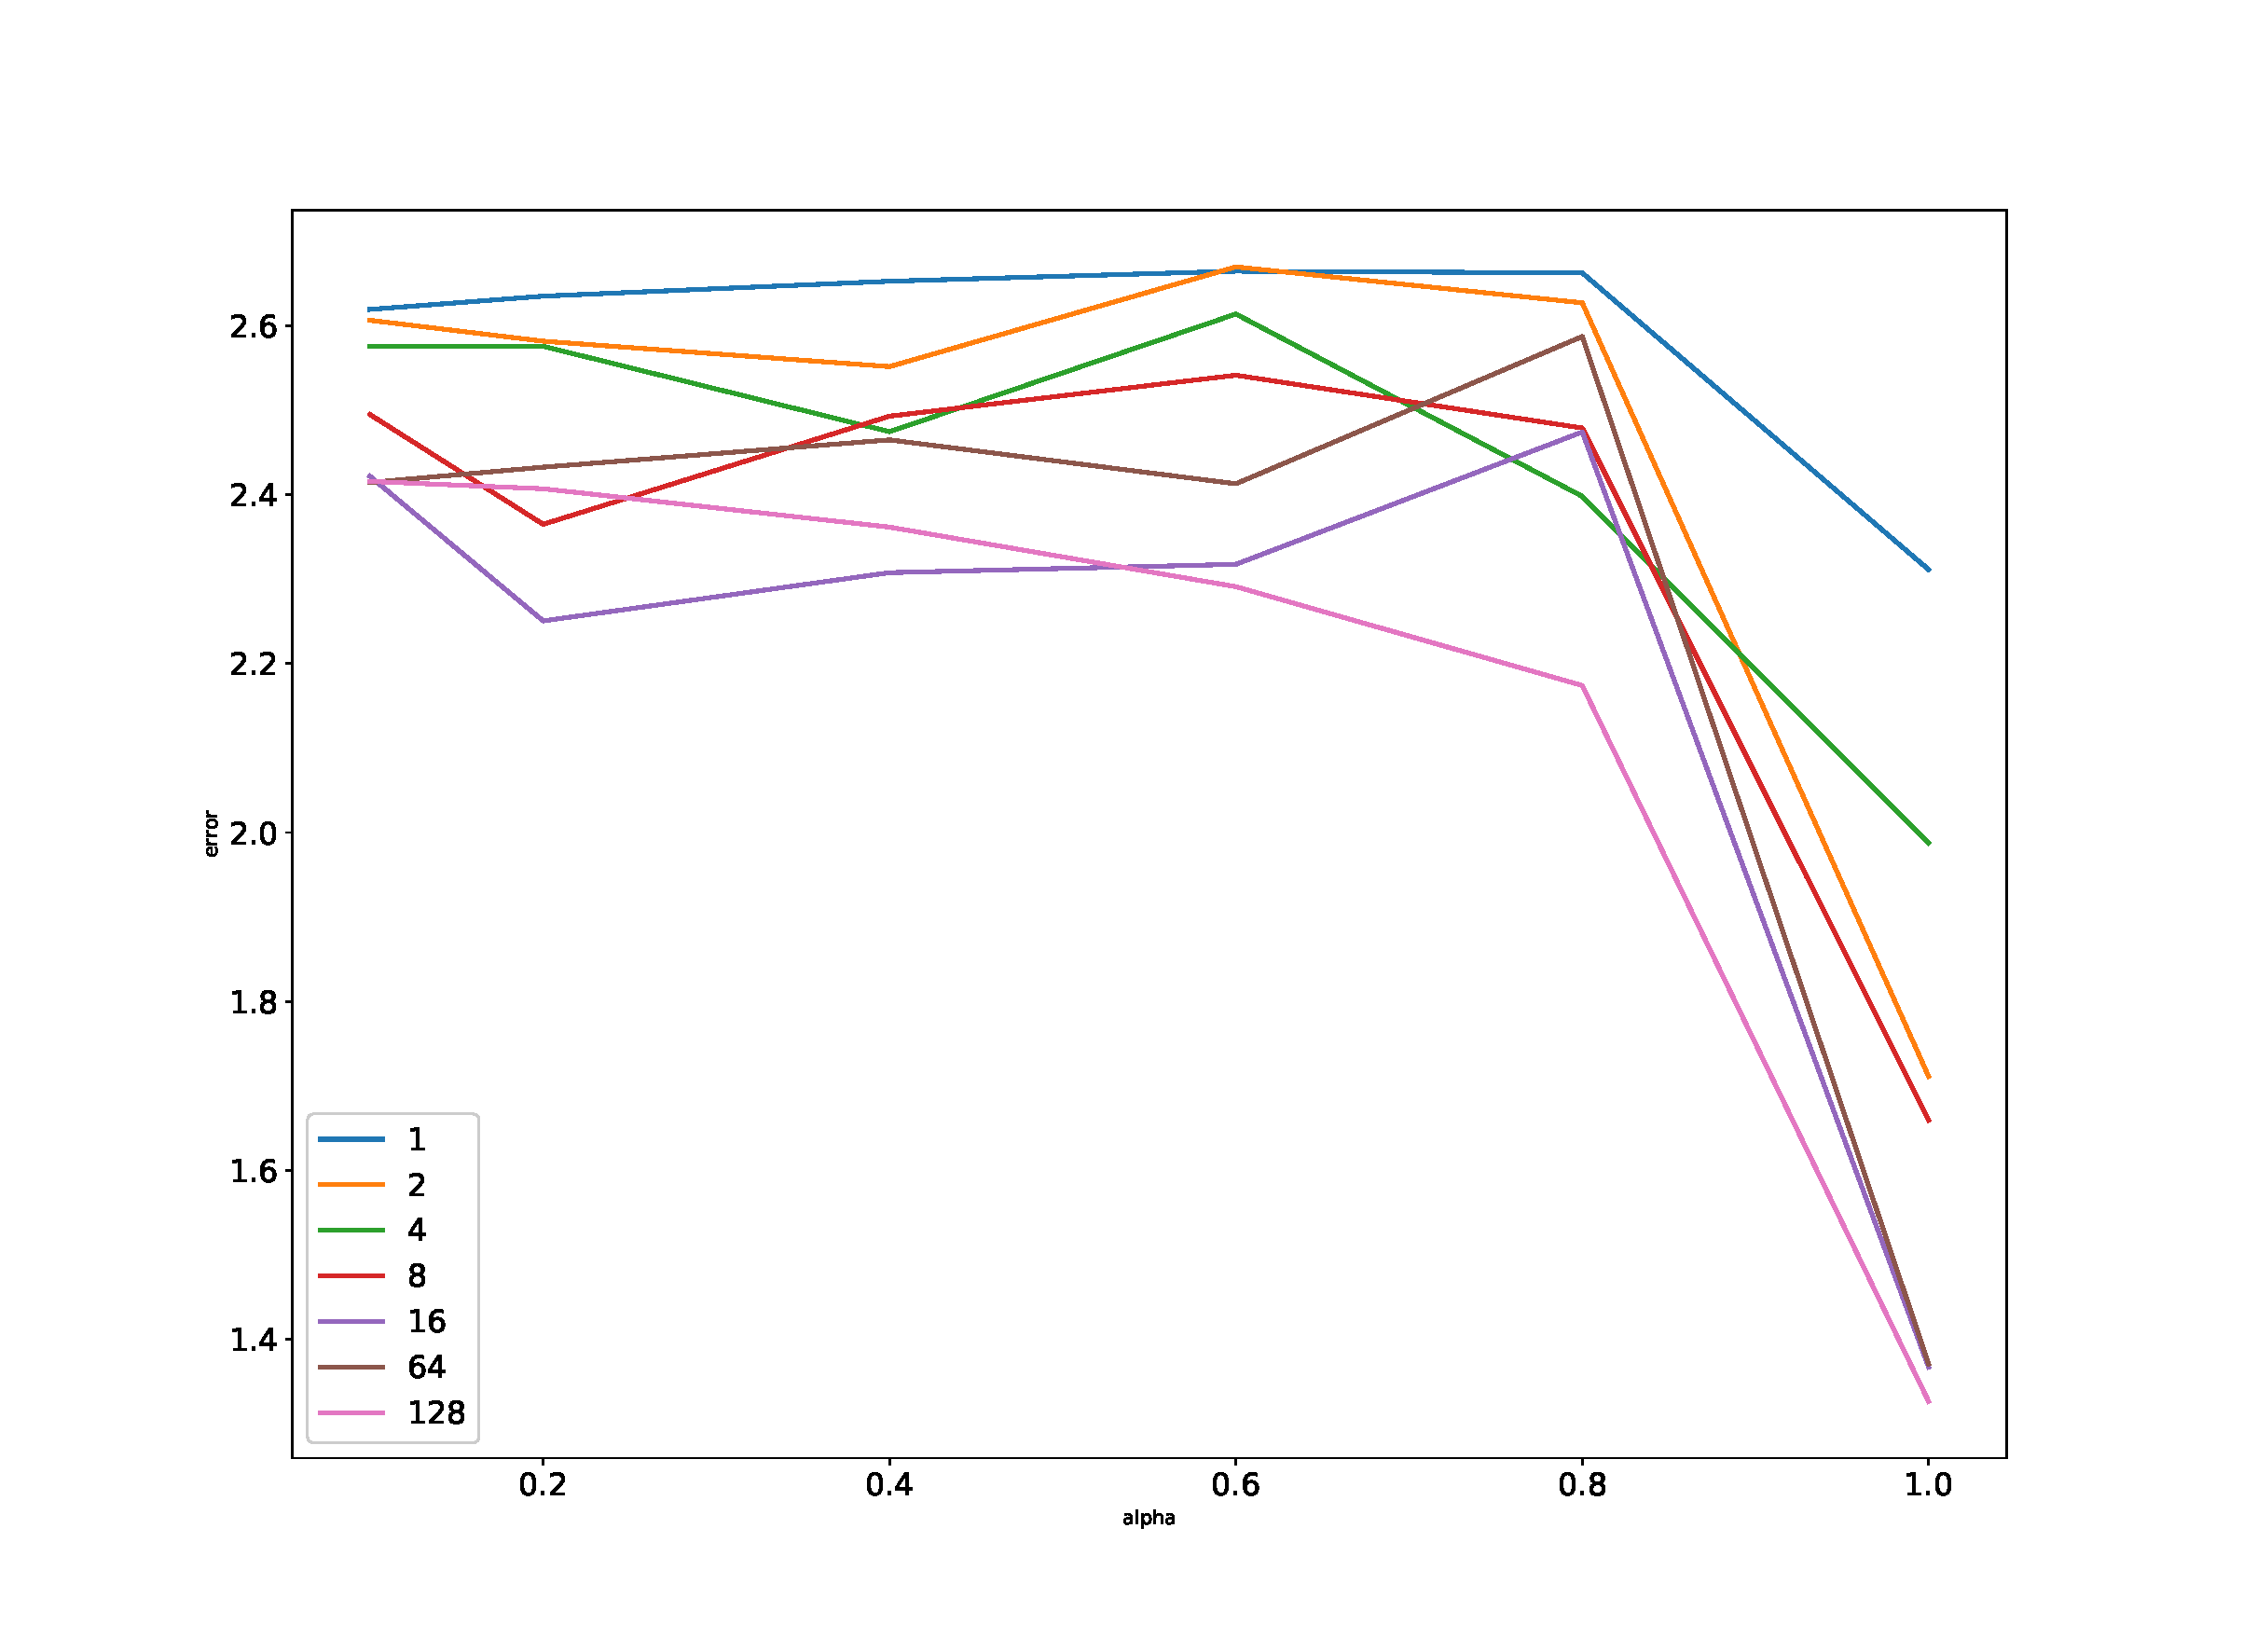
\includegraphics[width=.75\textwidth]{plots_v1.eps}
  \centering
  \caption{plot of n-sarsa performance}
  \label{fig1}
\end{figure}

\newpage


\begin{figure}[h!]
  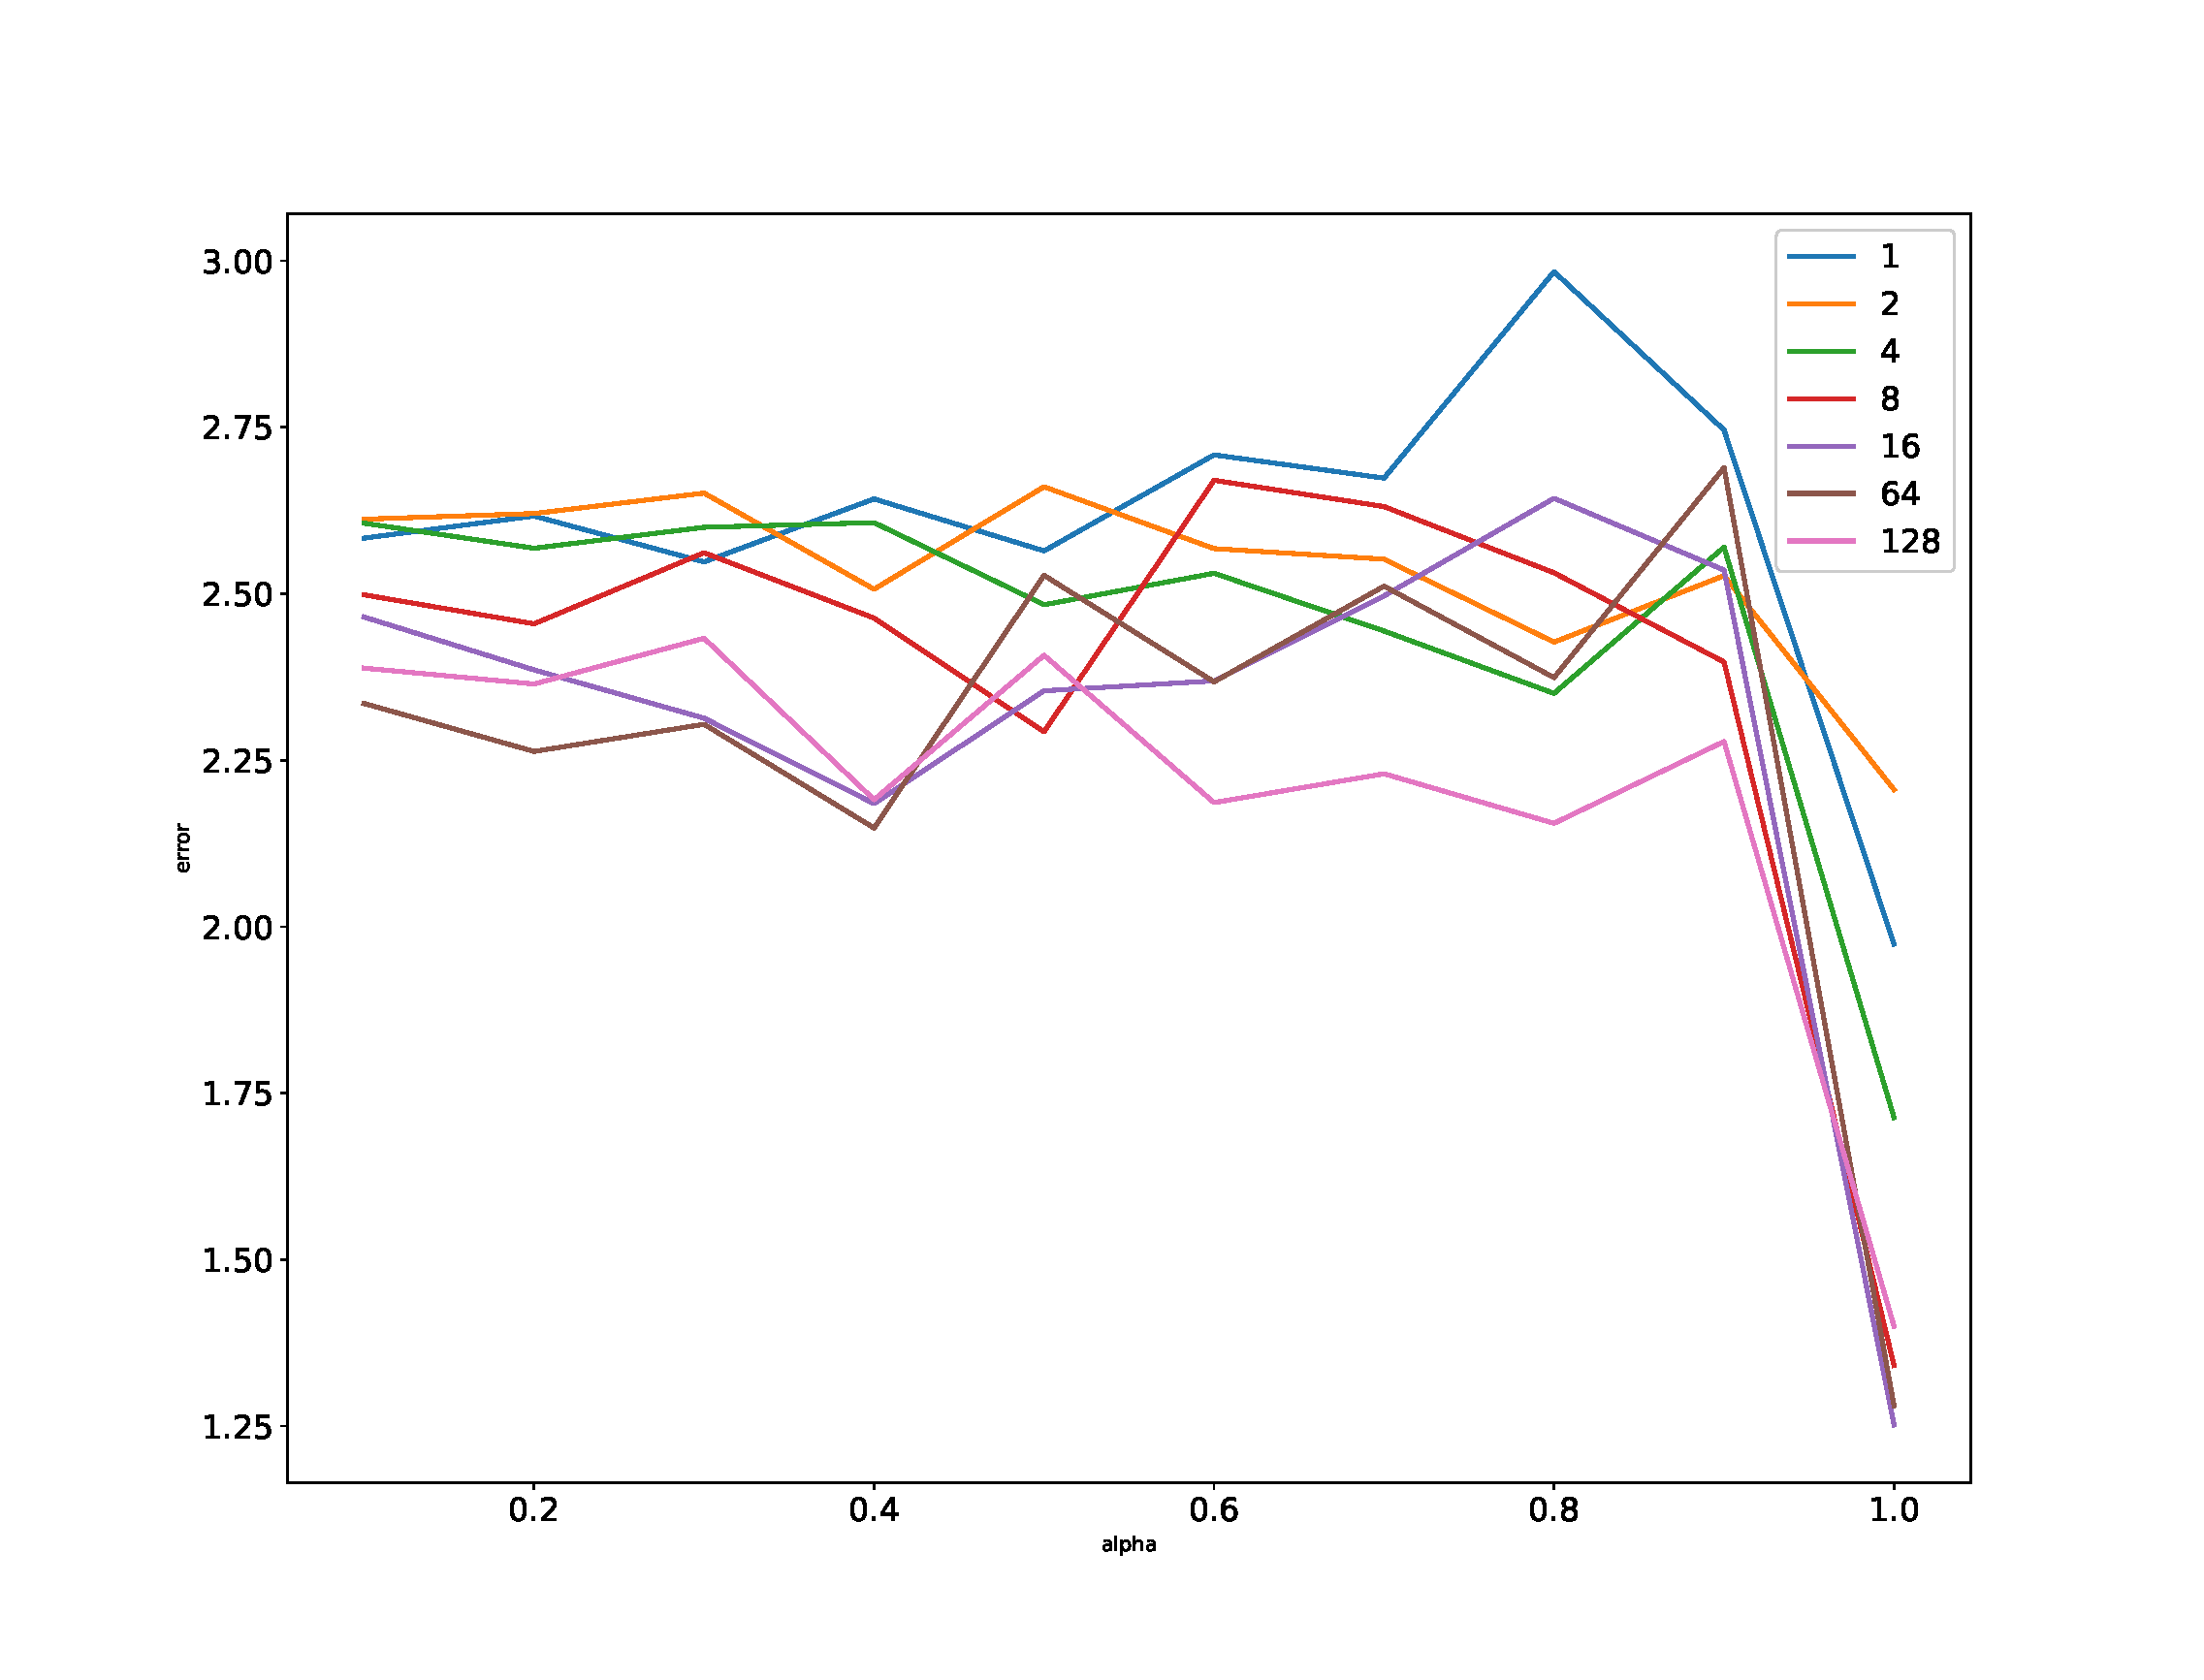
\includegraphics[width=.75\textwidth]{plots_v2.eps}
  \centering
  \caption{plot of n-sarsa performance}
  \label{fig2}
\end{figure}











\end{document}

